\documentclass[acmsmall,screen,review]{acmart}
\input{glyphtounicode}
\pdfgentounicode=1
\usepackage{tabularx}
\usepackage{xltabular}
\usepackage{longtable}
\usepackage{graphicx}
\usepackage{booktabs}
\usepackage{ragged2e}
\newcolumntype{Y}{>{\RaggedRight\arraybackslash}X}
\newcolumntype{Z}{>{\RaggedLeft\arraybackslash}X}
\settopmatter{printacmref=false}
\setcopyright{none}
\acmJournal{TQC}
\acmYear{2026}
\begin{document}
\renewcommand{\thesection}{S\arabic{section}}\renewcommand{\thetable}{S\arabic{table}}\renewcommand{\thefigure}{S\arabic{figure}}

\title{Supplementary Material: A Verifiable and Cost-Controlled Experiment Platform for Cloud Quantum Optimization Benchmarks}
\author{Hiroaki Tobita}
\affiliation{\institution{Advanced Institute of Industrial Technology}\city{Tokyo}\country{Japan}}
\email{tobita-hiroaki@aiit.ac.jp}
\begin{abstract}
This supplement holds three parts of the paper's record that a reader needs in order to reproduce or audit it, but not in order to follow it: the infrastructure footprint and the provider-side controls as of September 2026 (Section S1), the service-side task ledger behind the 177-task count of Table 7 of the main text (Section S2), and the commands every table of the main text came from, with what each took in wall-clock (Section S3), the three column-coverage passes (S4), the secondary analysis the record allowed (S5), the itemized cloud spend (S6), the stopping-stage figure (S7) and the detections by perturbation size (S8). Section, table and reference numbers without an S prefix refer to the main text; the two works cited here are listed at the end.
\end{abstract}
\ccsdesc[500]{Software and its engineering~Software verification and validation}
\ccsdesc[300]{Hardware~Quantum computation}
\ccsdesc[300]{Information systems~Data provenance}
\ccsdesc[300]{General and reference~Experimentation}

\keywords{reproducibility; experiment management; quantum cloud services}
\maketitle



\section{The CDK footprint}

Two stacks, region-pinned to \texttt{us-east-1} (Braket has no endpoint in the project's default region, which a first deployment discovered as a DNS failure before any task was submitted). \texttt{QfrBraketStack}: one S3 bucket (AES-256, public access blocked, SSL enforced, 90-day lifecycle) and one IAM role scoped to Braket and that bucket. \texttt{Qfr\allowbreak{}Monitoring\allowbreak{}Stack}: two Budgets, \$50 monthly and \$50 Braket-only, with notifications at 50/80/100\% actual and 100\% forecast. Three account-level preconditions are documented manual steps because no synthesis or test reveals them: the Braket service-linked role is not created on first use; the default region has no endpoint; the hardware provider's agreement is a console click. The retained footprint carries no idle charge. A per-QPU spending limit (\texttt{AWS:\allowbreak{}:\allowbreak{}Braket:\allowbreak{}:\allowbreak{}Spending\allowbreak{}Limit}) is a one-resource addition and is the ``both'' configuration of Section 5.2 as infrastructure; the stacks do not declare one, and the \$1.00 limit of Section 5.2 was created through the API for that observation and left in place, which a reader reproducing the observation should know: the account it was created on still refuses an IonQ task whose estimate exceeds \$1.00.


\subsection{Provider-side controls (Amazon Braket, as of September 2026)}


\begingroup
\small
\setlength\LTleft{\fill}
\setlength\LTright{\fill}
\begin{xltabular}{\textwidth}{>{\hsize=0.529\hsize}Y>{\hsize=2.228\hsize}Y>{\hsize=0.647\hsize}Y>{\hsize=0.588\hsize}Y>{\hsize=1.007\hsize}Y}
\caption{Four mechanisms, not one under four names: a per-device spending limit the provider operates, a sample deployment the customer runs, a budget that notifies, and a client-side timeout that bounds only how long the caller waits. Table 8's ``cap'' is the first; Table 9 measures the second.}\label{tab:1} \\
\toprule
\textbf{Kind} & \textbf{Control} & \textbf{Scope} & \textbf{When it acts} & \textbf{Observed here} \\
\midrule
\endfirsthead
\toprule
\textbf{Kind} & \textbf{Control} & \textbf{Scope} & \textbf{When it acts} & \textbf{Observed here} \\
\midrule
\endhead
\endfoot
\bottomrule
\endlastfoot
service, per device & spending limit (\texttt{Create\allowbreak{}Spending\allowbreak{}Limit}, Nov. 2025): rejects a task whose list-price estimate exceeds the remaining cap & on-demand QPU tasks only; the API refuses to create one for a simulator & at task creation & created (\$1.00 on IonQ Forte-1); the simulator refusal observed; the QPU rejection pending device availability (Sec. 5.2) \\
account, detective & AWS Budgets: notification at a threshold; optional action attaching an IAM deny & whole account & data lag of hours & deployed as notification only \\
account, detective & AWS Braket cost-control solution (May 2023) \cite{ref1}: EventBridge task-state events $\rightarrow$ Lambda $\rightarrow$ DynamoDB running cost $\rightarrow$ notification or IAM deny on \texttt{braket:\allowbreak{}Create\allowbreak{}Quantum\allowbreak{}Task} & simulators, QPUs, hybrid jobs & near real time; ``a few'' tasks may be created before the denial propagates & deployed for Sec. 5.2 and destroyed: as documented it metered nothing (400 tasks passed); fixed, five runs denied 41--92 tasks (median 47) past the limit, 6--56 (median 10) past the alarm \\
client, not a charge control & \texttt{poll\_\allowbreak{}timeout\_\allowbreak{}seconds} of the PennyLane--Braket device. In \texttt{Aws\allowbreak{}Quantum\allowbreak{}Task.\allowbreak{}\_\allowbreak{}wait\_\allowbreak{}for\_\allowbreak{}completion} (SDK 1.125) the timeout ends the polling loop, logs a warning and returns \texttt{None}; the task keeps running on the service and keeps accruing its charge. Cancelling is a separate call, \texttt{Aws\allowbreak{}Quantum\allowbreak{}Task.\allowbreak{}cancel()} & the caller's process, waiting for one task & while waiting for a result & set to 3,600 s here against the library's 432,000 s (five-day) default; nothing in this project reached it \\
\end{xltabular}
\endgroup


\subsection{The cost-control deployment}

Upstream commit \texttt{19eaad6} of \texttt{aws-\allowbreak{}samples/\allowbreak{}cost-\allowbreak{}control-\allowbreak{}for-\allowbreak{}amazon-\allowbreak{}braket}, deployed 2026-09-17 in \texttt{us-east-1} only with a \$0.30 monthly and \$3 all-time limit and the denial targeted at the project's IAM user, then destroyed. Three changes, kept as a patch in the repository (\texttt{cdk/\allowbreak{}cost\_\allowbreak{}control\_\allowbreak{}patch/\allowbreak{}}): Lambda images built for x86\_64 rather than arm64 (the build host has no arm64 emulation); \texttt{NUMBA\_\allowbreak{}CACHE\_\allowbreak{}DIR=/\allowbreak{}tmp/\allowbreak{}numba} on the task-logger function, without which the function fails on import; and, for the repetitions only, the monthly alarm's evaluation window shortened from 24 h to 5 min so that a cleared running cost lets the alarm return to OK between runs (\texttt{datapoints\_\allowbreak{}to\_\allowbreak{}alarm} stays 1, so the latency to ALARM is unchanged). Between runs the denial was detached by hand --- the sample detaches only on a transition to OK --- and the running-cost table emptied. The stacks create an EventBridge bus and two rules, five Lambda functions, two DynamoDB tables, seven CloudWatch alarms, a dashboard, an SNS topic and one managed policy (\texttt{Deny braket:\allowbreak{}Create\allowbreak{}Quantum\allowbreak{}Task}). Destroying them requires detaching that policy from the controlled identities first and deleting the event-bus stack last.


\section{The task ledger}

\texttt{sv1\_\allowbreak{}task\_\allowbreak{}ledger.\allowbreak{}py} groups the archived SV1 task records (1,299 tasks) into runs by submission time and counts analytic against sampling tasks. Run 1 (2026-08-09, N = 8 pilot): 227 tasks, 50 analytic and 177 sampling, 177,000 shots. Run 2 (the same after \texttt{frozen\_angles}): 204 tasks for four sizes, 200 analytic and 4 sampling. The ledger is the service-side member of the three-way agreement of Table 7.


\section{Reproduction commands for the main text}

These are the commands the tables came from, with what each took in wall-clock. The first group runs on a CPU and bills nothing: a reader who wants to re-derive one table runs one of these, and \texttt{es3\_\allowbreak{}reconstruction.\allowbreak{}py} is the one that plays the reader (Section 5.3 reports what it costs). The two at the end bill the account they are run in and create a spending limit in it; they are recorded so that a reader knows what produced the cells Table 8 marks as observed on the service, not so that the reader repeats them.


\begin{small}\begin{verbatim}
# ~12 min, CPU
python -m experiments.system_paper.es1_fault_injection
# ~25 min: the same thirteen checks on the five committed clean records
python -m experiments.system_paper.es1_fault_injection --clean-records
# ~2.5 h: column coverage (133 columns) + 300 random mutations
# (both need the per-run artifacts: e1_runs*.npz, about 100 MB, from the Zenodo deposit
#  of the numerical study, doi:10.5281/zenodo.24032941)
python -m experiments.system_paper.es1_random_faults --faults 300
# ~1.8 h: the held-out draw, after the relations were frozen (last row of Table 4)
python -m experiments.system_paper.es1_random_faults --faults 300 \
    --seed 7 --tag heldout --no-coverage
# ~1 h each: the same on a sibling record (--record _e5 or _e3_lbfgs; outputs carry the suffix)
python -m experiments.system_paper.es1_fault_injection --record _e5
python -m experiments.system_paper.es1_random_faults --record _e5 --faults 300 --tag e5
python -m experiments.system_paper.es1_random_faults --record _e5 --faults 300 \
    --seed 7 --tag e5_heldout --no-coverage
python -m experiments.system_paper.es1_tiers --record _e5
# ~1.8 h (N = 20 is 94 min of tape construction); --sizes 8 runs in 1 min
python -m experiments.system_paper.es2_guard_stages
# Table 9 from the committed task records of the six runs (seconds, no AWS)
python -m experiments.system_paper.es2_cost_control_aggregate
# ~15 min with a warm pip cache; clones the public package
python -m experiments.system_paper.es3_reconstruction
# ~7 min: the v1.2 block of Table 10 (the archived release)
python -m experiments.system_paper.es3_reconstruction --tag v1.2 --out-suffix _v12 \
    --only clone venv tests level1 level2 status
# ~4 min: level 3 on v1.2, the 24-run block of Table 10 and its column agreement
python -m experiments.system_paper.es3_reconstruction --tag v1.2 --out-suffix _v12level3 \
    --only clone venv level3
# seconds: the tier count of Table 5 from the detection matrix, the mutation files and the
# clause-source replays (es1_clause_sources.py, ~2.5 h on the main record, ~20 min on a sibling)
python -m experiments.system_paper.es1_clause_sources --injected
python -m experiments.system_paper.es1_clause_sources --seed 2026 --faults 300
python -m experiments.system_paper.es1_clause_sources --seed 7 --faults 300 --skip-coverage \
    --tag _heldout --expect-tag _heldout
python -m experiments.system_paper.es1_tiers
# seconds each: the declarative control run as the library it stands for (Section 5.1).
# Needs requirements-control.txt; the mutation replay refuses to write unless it
# reproduces the committed stream.
python -m experiments.system_paper.es1_pandera_compare
python -m experiments.system_paper.es1_pandera_mutations --faults 300 --seed 2026
python -m experiments.system_paper.es1_pandera_mutations --faults 300 --seed 7 \
    --skip-coverage --expect-tag _heldout --tag _heldout
python -m experiments.system_paper.es1_pandera_compare --record _e5
python -m experiments.system_paper.es1_pandera_mutations --record _e5 --faults 300 \
    --seed 2026 --expect-tag _e5 --tag _e5
python -m pytest -q tests/test_es1_fault_injection.py tests/test_es1_random_faults.py \
    tests/test_es2_guard_stages.py tests/test_es2_cost_control_aggregate.py \
    tests/test_es3_reconstruction.py tests/test_run_status.py \
    tests/test_es1_pandera_control.py

# The two that bill. Each creates tasks in the account whose credentials it finds, and the
# first also creates a $1.00 spending limit on IonQ Forte-1. Nothing above needs either.
# the sampling fallback re-observed on SV1 (~$0.67) and the spending-limit request
python -m experiments.system_paper.es2_observe_cloud --s3-bucket <bucket> --yes-bill-me
# one repetition of the account-level control, after deploying cdk/cost_control_patch/
# (up to --max-tasks tasks, 400 by default, ~$1.50 on SV1)
python -m experiments.system_paper.es2_observe_cost_control --s3-bucket <bucket> --yes-bill-me
\end{verbatim}\end{small}

\section{The column-coverage passes}

The column coverage of Section 5.1 of the main text was scanned three times, because the first pass's uncovered list told us which columns a further identity could bind; the relations were developed against the first two passes and the third is the final one. Four columns (\texttt{p\_layers}, \texttt{steps}, \texttt{stepsize}, \texttt{status}) were bound in the second pass by adding them to the manifest relation's list of columns that must hold one value across the file, which is why the last column of the table is smaller than the increase: 47 + 4 + 52 = 103 and 47 + 4 + 63 = 114.



\begingroup
\small
\setlength\LTleft{\fill}
\setlength\LTright{\fill}
\begin{xltabular}{\textwidth}{rYrr}
\caption{Column coverage of the relations over the 133 columns of the run row, the reference row and the artifact; the one column empty on every row is excluded. Each pass is a committed scan of the whole record. The last column counts the columns no other relation binds.}\label{tab:2} \\
\toprule
\textbf{Pass} & \textbf{Checks} & \textbf{Covered} & \textbf{Covered by \texttt{identities} alone} \\
\midrule
\endfirsthead
\toprule
\textbf{Pass} & \textbf{Checks} & \textbf{Covered} & \textbf{Covered by \texttt{identities} alone} \\
\midrule
\endhead
\endfoot
\bottomrule
\endlastfoot
1 & 12 relations without the identity check & 47 / 132 & 0 \\*
2 & + identities ($Q_{\tau}$, $P_{\tau}$/$P_{\mathrm{opt}}$, rank, D and the offset magnitude, best expectation, uniform baselines, Sharpe constancy) & 103 / 132 & 52 \\*
3 & + shot-level successes, fractions, distinct shots, probability sums, portfolio metrics from the pinned statistics, reference row against its own cardinality minima and stored f & 114 / 132 & 63 \\
\end{xltabular}
\endgroup


\section{Secondary analysis from the record}

A record bound to its inputs (P1) has a use the three evaluations do not measure: it answers questions that were not asked when it was written. Two such questions arose while planning the work that follows this paper --- whether a stored portfolio survives a change of market window, risk aversion, cardinality or universe, and what a second, sector-level constraint does to the problem of \cite{ref1} --- and both were settled from the committed record alone, in minutes of CPU, with no quantum run and no cloud task, because the record carries the best feasible portfolio of every run, the stored final state, and the enumerated feasible set of every instance. The answers are about portfolios and belong to the studies they re-scoped, not here. What belongs here is their cost and their check. Both were checked the way Section 4.1 checks the record: re-scoring the stored portfolios under \textit{unchanged} conditions reproduced the recorded $g_{F}$, rank and f on all 826 rows with no mismatch; the enumerated objective agreed with every stored feasible-set value to 2$\cdot$10$^{-16}$; and the single-constraint critical weight recomputed by the new code equalled the reference file's on all 30 instances. The scripts and their result files are in the package (\texttt{experiments/\allowbreak{}a1\_\allowbreak{}reuse/\allowbreak{}}, \texttt{experiments/\allowbreak{}a3\_\allowbreak{}constraints/\allowbreak{}}). Two studies were re-scoped in minutes, because every run was already bound to its inputs and to an exact reference, and the re-scoring could be checked against values the record already held.


\section{The cloud spend}


\begingroup
\small
\setlength\LTleft{\fill}
\setlength\LTright{\fill}
\begin{xltabular}{\textwidth}{Yll}
\caption{Cloud tasks paid for, by what they were paid for. Each cost is the row's task count at SV1's \$0.00375 per task --- the three-second minimum --- rounded to the cent, and \textit{this paper}'s total is the sum of those rounded figures; the rounded sum of 1,249 tasks is \$4.68. The last two rows are the provider's billing console and are not derived from a count.}\label{tab:3} \\
\toprule
\textbf{What} & \textbf{Tasks} & \textbf{Cost} \\
\midrule
\endfirsthead
\toprule
\textbf{What} & \textbf{Tasks} & \textbf{Cost} \\
\midrule
\endhead
\endfoot
\bottomrule
\endlastfoot
the sampling-fallback observation on SV1 (Section 5.2) & 178 & \$0.67 \\*
the account-level cost control as documented, the deployment that metered nothing (Section 5.2) & 400 & \$1.50 \\*
the same control with its import fixed, the five repetitions of Table 9 of the main text & 671 & \$2.52 \\*
the IonQ spending-limit probe: limit created, device never online (Section 5.2) & 0 & \$0.00 \\*
\textbf{this paper} & \textbf{1,249} & \textbf{\$4.69} \\*
the numerical study \cite{ref1}: SV1 and IonQ arms, 2026-08 to 2026-09 & --- & \$37.90 \\*
\textbf{the project on Amazon Braket, to date} & --- & \textbf{\$42.59} \\
\end{xltabular}
\endgroup


\section{Where each misconfiguration stops, as a figure}

The figure draws the N = 8 cells of Table 8 of the main text: the stage at which each misconfiguration stops under each of the four guard configurations, with the list-price bill.


\begin{figure}[t]
\centering
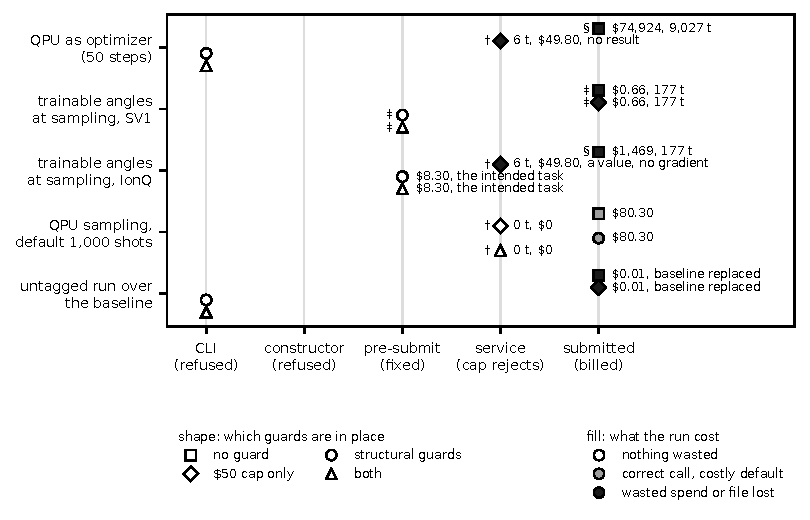
\includegraphics[width=\textwidth]{figures/fig_guard_stages.pdf}
\caption{Where each misconfiguration stops under the four guard configurations (N = 8, list prices). Nothing is carried by colour: the marker's shape is the guard configuration and its fill the outcome --- open for nothing wasted, grey for a correct call with a costly default, solid for wasted spend or the baseline file lost. Provenance marks as in Table 8 of the main text: $\ddagger$ observed on Amazon Braket, \S{} counted as circuits and converted at one task per circuit, $\dagger$ the provider's documented behaviour; t = tasks.}
\label{fig:1}
\end{figure}


\section{Detection by the magnitude of a perturbation}

Section 5.1 of the main text states the relations' detection rate by the size of the perturbation. Table~S4 gives the counts behind it, for both draws, over every operator that perturbs a value --- a run-table cell, a reference cell, an artifact element or a derived statistic; a count can only move by $\pm$1, and those are the first row.



\begingroup
\small
\setlength\LTleft{\fill}
\setlength\LTright{\fill}
\begin{xltabular}{\textwidth}{Yrrrr}
\caption{Random perturbations by magnitude, both draws: how many were drawn and how many the relations detected. 10$^{-9}$ is the relative tolerance of the numerical relations.}\label{tab:4} \\
\toprule
\textbf{Magnitude} & \textbf{Main draw: n} & \textbf{Main draw: detected} & \textbf{Held-out: n} & \textbf{Held-out: detected} \\
\midrule
\endfirsthead
\toprule
\textbf{Magnitude} & \textbf{Main draw: n} & \textbf{Main draw: detected} & \textbf{Held-out: n} & \textbf{Held-out: detected} \\
\midrule
\endhead
\endfoot
\bottomrule
\endlastfoot
$\pm$1 (a count) & 5 & 5 (100\%) & 5 & 5 (100\%) \\*
10$^{-9}$ & 51 & 24 (47\%) & 32 & 16 (50\%) \\*
10$^{-6}$ & 38 & 30 (79\%) & 53 & 47 (89\%) \\*
10$^{-3}$ & 42 & 34 (81\%) & 46 & 34 (74\%) \\*
10$^{-1}$ & 46 & 37 (80\%) & 51 & 44 (86\%) \\
\end{xltabular}
\endgroup


\begin{thebibliography}{99}
\bibitem{ref1} Amazon Web Services, \texttt{aws-\allowbreak{}samples/\allowbreak{}cost-\allowbreak{}control-\allowbreak{}for-\allowbreak{}amazon-\allowbreak{}braket}, commit \texttt{19eaad6}, accessed 27 Sep. 2026: EventBridge task-state events, Lambda, DynamoDB, CloudWatch and an IAM deny on \texttt{braket:\allowbreak{}Create\allowbreak{}Quantum\allowbreak{}Task} (announced on the AWS Quantum Technologies Blog, 31 May 2023). The deployment measured in Section 5.2 of the main text is of that commit.
\end{thebibliography}
\end{document}
